\section{Introduction to machine learning}

\begin{frame}{Introduction}
    \begin{tikzpicture}
        \node[draw=black] at (-5.25, -3.5) {};
        \node[draw=black] at (5.25, 3.5) {};
        \visible<1-2>{
            \node[text width=10.5cm] at (0, 0) {
                \textbf{Key terminology:}
                \begin{itemize}
                    \item Statistical learning: A set of tools (often called models) for understanding data
                    \item<2> Supervised learning: We know what task we want to solve
                    \item<2> Unsupervised learning: We don't know what task we want to solve (or we don't have the data we need to solve it)
                \end{itemize}
            };
        }
        \visible<3-4,6-7>{

            \node[inner sep=0pt, draw=black, anchor=west] (x1) at (-5.25, 2.5) {
                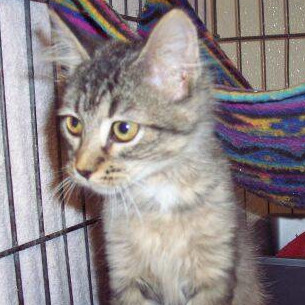
\includegraphics[width=1cm]{data/cats_and_dogs/cat.2.jpg}
            };
            \node[inner sep=0pt, draw=black] (x2) at ($ (x1) - (0, 1.5) $) {
                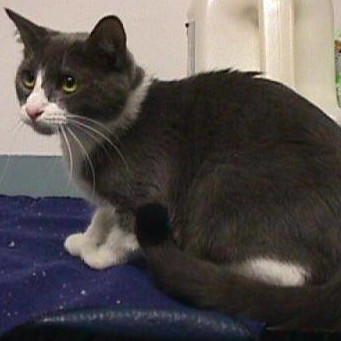
\includegraphics[width=1cm]{data/cats_and_dogs/cat.0.jpg}
            };
            \node[inner sep=0pt, draw=black] (x3) at ($ (x1) - (0, 3) $) {
                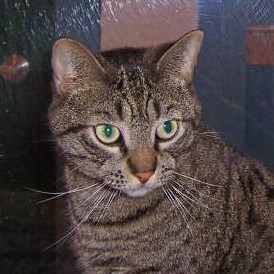
\includegraphics[width=1cm]{data/cats_and_dogs/cat.1.jpg}
            };
            \node[inner sep=0pt, draw=black] (x3) at ($ (x1) - (0, 4.5) $) {
                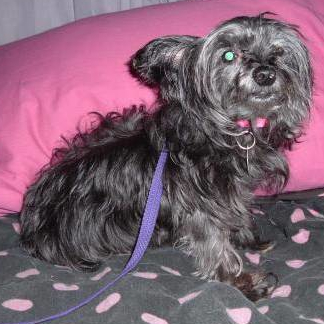
\includegraphics[width=1cm]{data/cats_and_dogs/dog.0.jpg}
            };

            \node[inner sep=0pt, draw=black] (x5) at ($ (x1) - (-1.25, 0.75) $) {
                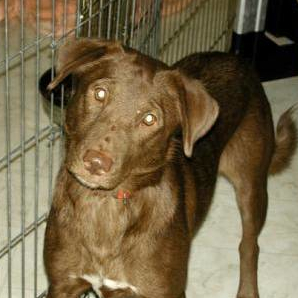
\includegraphics[width=1cm]{data/cats_and_dogs/dog.1.jpg}
            };
            \node[inner sep=0pt, draw=black] (x6) at ($ (x1) - (-1.25, 2.25) $) {
                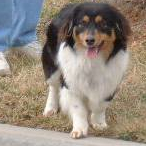
\includegraphics[width=1cm]{data/cats_and_dogs/dog.2.jpg}
            };
            \node[inner sep=0pt, draw=black] (x7) at ($ (x1) - (-1.25, 3.75) $) {
                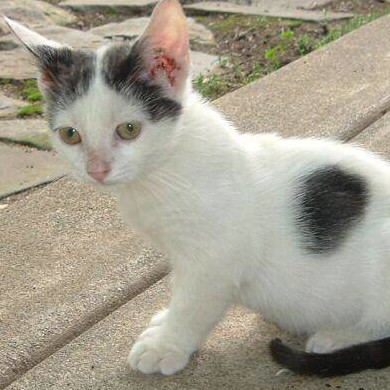
\includegraphics[width=1cm]{data/cats_and_dogs/cat.3.jpg}
            };
        }
        \visible<5>{
            \node[inner sep=0pt, draw=black, anchor=west, label=below:\tiny{Cat}] (x1) at (-5.25, 2.5) {
                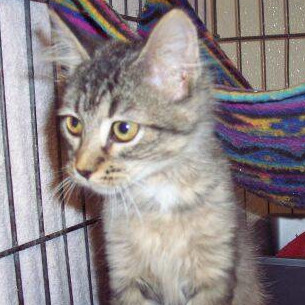
\includegraphics[width=1cm]{data/cats_and_dogs/cat.2.jpg}
            };
            \node[inner sep=0pt, draw=black, label=below:\tiny{Cat}] (x2) at ($ (x1) - (0, 1.5) $) {
                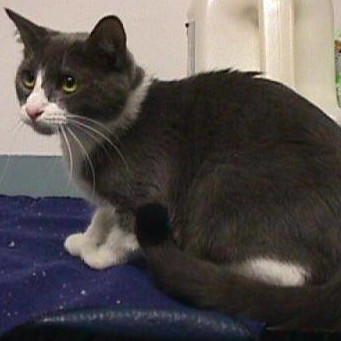
\includegraphics[width=1cm]{data/cats_and_dogs/cat.0.jpg}
            };
            \node[inner sep=0pt, draw=black, label=below:\tiny{Cat}] (x3) at ($ (x1) - (0, 3) $) {
                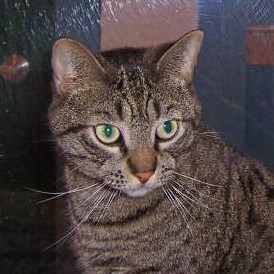
\includegraphics[width=1cm]{data/cats_and_dogs/cat.1.jpg}
            };
            \node[inner sep=0pt, draw=black, label=below:\tiny{Dog}] (x3) at ($ (x1) - (0, 4.5) $) {
                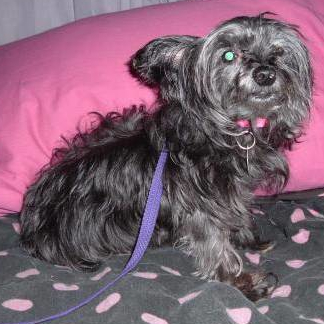
\includegraphics[width=1cm]{data/cats_and_dogs/dog.0.jpg}
            };

            \node[inner sep=0pt, draw=black, label=below:\tiny{Dog}] (x5) at ($ (x1) - (-1.25, 0.75) $) {
                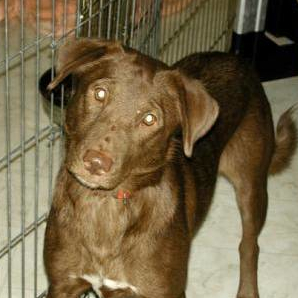
\includegraphics[width=1cm]{data/cats_and_dogs/dog.1.jpg}
            };
            \node[inner sep=0pt, draw=black, label=below:\tiny{Dog}] (x6) at ($ (x1) - (-1.25, 2.25) $) {
                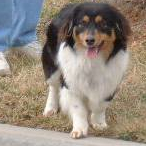
\includegraphics[width=1cm]{data/cats_and_dogs/dog.2.jpg}
            };
            \node[inner sep=0pt, draw=black, label=below:\tiny{Cat}] (x7) at ($ (x1) - (-1.25, 3.75) $) {
                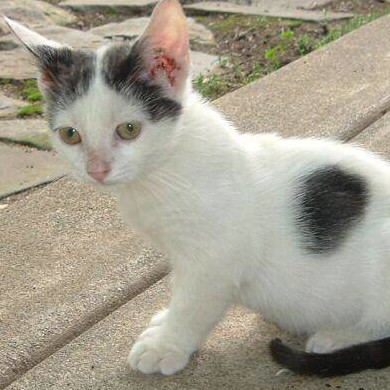
\includegraphics[width=1cm]{data/cats_and_dogs/cat.3.jpg}
            };
        }
        \visible<4-5>{

            \node[align=center, font=\scriptsize, draw=black] (sm) at ($ (x1) + (3.5, -0.75) $) {
                Supervised\\model
            };
            \draw[-stealth, gray!50, line width=3pt] (x6) to [in=270, out=0] (sm);
            \draw[-stealth, gray!50, line width=3pt] (sm) -- ($ (sm.east) + (1.1, 0) $);

            \node[inner sep=0pt, draw=black] (y1) at ($ (sm.center) + (5, 0.5) $) {
                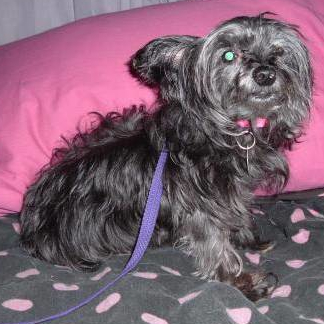
\includegraphics[width=1cm]{data/cats_and_dogs/dog.0.jpg}
            };
            \node[anchor=west, inner sep=0pt, draw=black] (y2) at (y1.east) {
                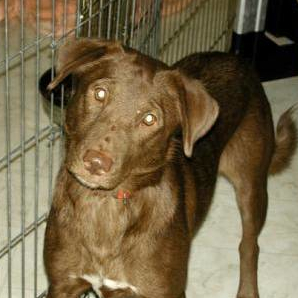
\includegraphics[width=1cm]{data/cats_and_dogs/dog.1.jpg}
            };
            \node[anchor=north, inner sep=0pt, draw=black] at (y1.south) {
                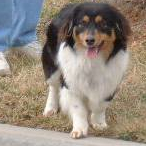
\includegraphics[width=1cm]{data/cats_and_dogs/dog.2.jpg}
            };

            \node[inner sep=0pt, draw=black] (y4) at ($ (sm) + (2.5, 0.5) $) {
                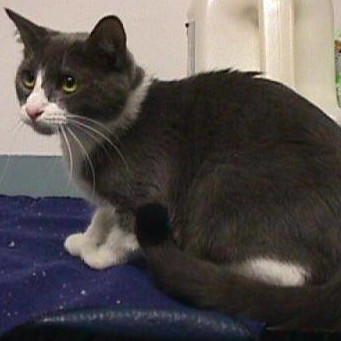
\includegraphics[width=1cm]{data/cats_and_dogs/cat.0.jpg}
            };
            \node[anchor=west, inner sep=0pt, draw=black] (y5) at (y4.east) {
                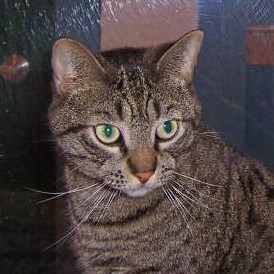
\includegraphics[width=1cm]{data/cats_and_dogs/cat.1.jpg}
            };
            \node[anchor=north, inner sep=0pt, draw=black] (y6) at (y4.south) {
                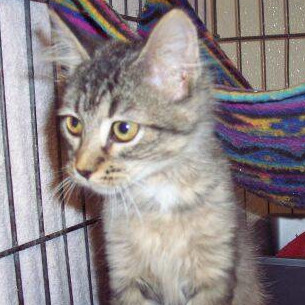
\includegraphics[width=1cm]{data/cats_and_dogs/cat.2.jpg}
            };
            \node[anchor=north, inner sep=0pt, draw=black] (y7) at (y5.south) {
                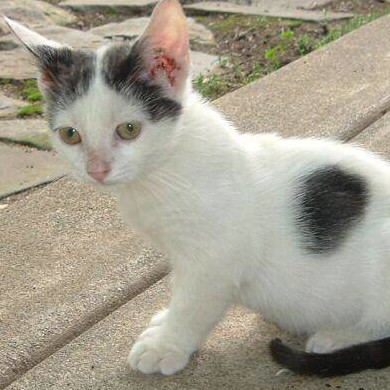
\includegraphics[width=1cm]{data/cats_and_dogs/cat.3.jpg}
            };

            \node[anchor=south, text depth=0] at ($ (y1.north)!0.5!(y2.north) $) {
                Dogs
            };
            \node[anchor=south, text depth=0] at ($ (y4.north)!0.5!(y5.north) $) {
                Cats
            };
        }
        \visible<6-7>{

            \node[align=center, font=\scriptsize, draw=black] (um) at ($ (x1) + (3.5, -3.75) $) {
                Unsupervised\\model
            };
            \draw[-stealth, gray!50, line width=3pt] (x6) to [in=90, out=0] (um);
            \draw[-stealth, gray!50, line width=3pt] (um) -- ($ (um.east) + (1.1, 0) $);
        }
        \visible<6>{
            \node[inner sep=0pt, draw=black] at ($ (um.center) + (6, 0.55) $) {
                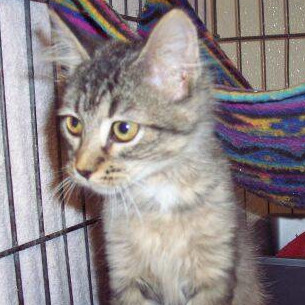
\includegraphics[width=1cm]{data/cats_and_dogs/cat.2.jpg}
            };
            \node[inner sep=0pt, draw=black] at ($ (um.center) + (5.95, -0.65) $) {
                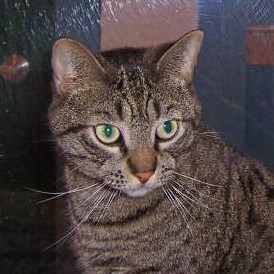
\includegraphics[width=1cm]{data/cats_and_dogs/cat.1.jpg}
            };
            \node[inner sep=0pt, draw=black] at ($ (um.center) + (4.8, 0.4) $) {
                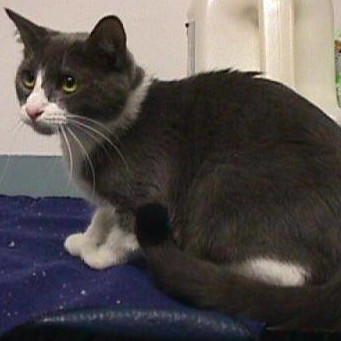
\includegraphics[width=1cm]{data/cats_and_dogs/cat.0.jpg}
            };
            \node[inner sep=0pt, draw=black] at ($ (um.center) + (4.7, -0.7) $) {
                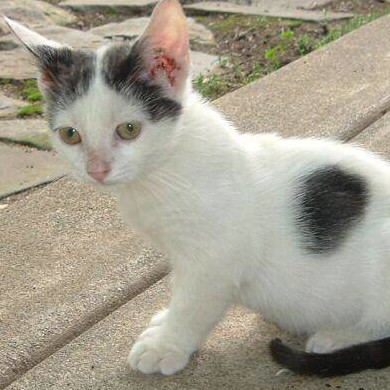
\includegraphics[width=1cm]{data/cats_and_dogs/cat.3.jpg}
            };

            \node[inner sep=0pt, draw=black] at ($ (um.center) + (2.7, 1.2) $) {
                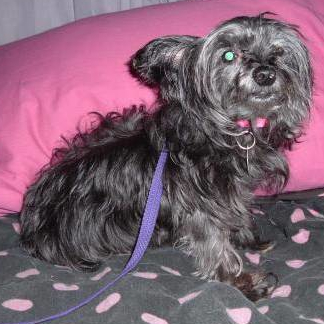
\includegraphics[width=1cm]{data/cats_and_dogs/dog.0.jpg}
            };
            \node[inner sep=0pt, draw=black] at ($ (um.center) + (2.55, 0) $) {
                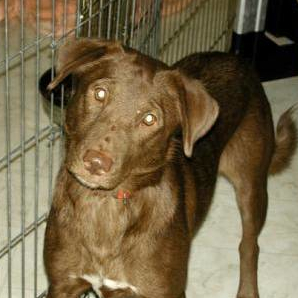
\includegraphics[width=1cm]{data/cats_and_dogs/dog.1.jpg}
            };
            \node[inner sep=0pt, draw=black] at ($ (um.center) + (2.65, -1.1) $) {
                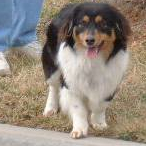
\includegraphics[width=1cm]{data/cats_and_dogs/dog.2.jpg}
            };
        }
        \visible<7>{
            \node[inner sep=0pt, draw=black] at ($ (um.center) + (6, 0.55) $) {
                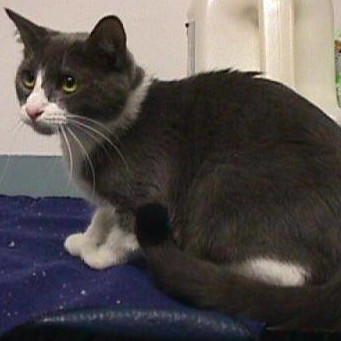
\includegraphics[width=1cm]{data/cats_and_dogs/cat.0.jpg}
            };
            \node[inner sep=0pt, draw=black] at ($ (um.center) + (5.95, -0.65) $) {
                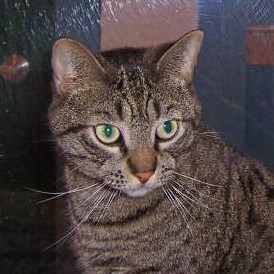
\includegraphics[width=1cm]{data/cats_and_dogs/cat.1.jpg}
            };
            \node[inner sep=0pt, draw=black] at ($ (um.center) + (4.8, 0.4) $) {
                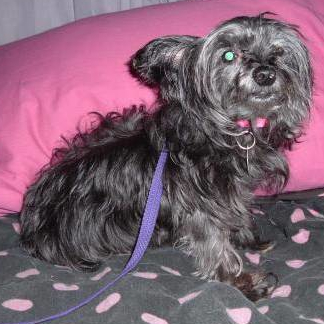
\includegraphics[width=1cm]{data/cats_and_dogs/dog.0.jpg}
            };
            \node[inner sep=0pt, draw=black] at ($ (um.center) + (4.7, -0.7) $) {
                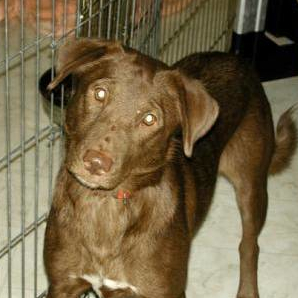
\includegraphics[width=1cm]{data/cats_and_dogs/dog.1.jpg}
            };

            \node[inner sep=0pt, draw=black] at ($ (um.center) + (2.7, 1.2) $) {
                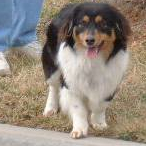
\includegraphics[width=1cm]{data/cats_and_dogs/dog.2.jpg}
            };
            \node[inner sep=0pt, draw=black] at ($ (um.center) + (2.55, 0) $) {
                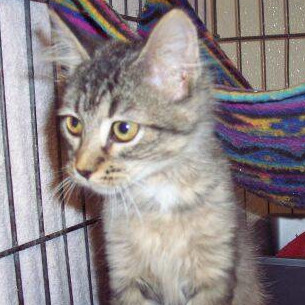
\includegraphics[width=1cm]{data/cats_and_dogs/cat.2.jpg}
            };
            \node[inner sep=0pt, draw=black] at ($ (um.center) + (2.65, -1.1) $) {
                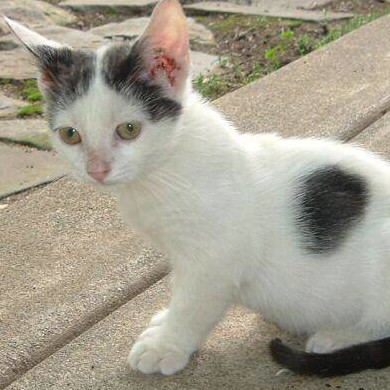
\includegraphics[width=1cm]{data/cats_and_dogs/cat.3.jpg}
            };
        }

    \end{tikzpicture}
\end{frame}

\newcommand{\mpgvsweight}[1]{
    \begin{tikzpicture}
        \begin{axis}[
            height=4cm,
            width=10cm,
            xlabel=$x$ (weight),
            ylabel=$y$ (mpg),
            ytick pos=left,
            xtick pos=bottom,
            xmin=30,
            xmax=245,
            ymin=6,
            ymax=51
        ]

        \addplot[
            only marks,
            cyan,
            opacity=0.5
        ] table [
            col sep=comma,
            x=horsepower,
            y=mpg
        ] {data/Auto.csv};

        \ifnum#1=1
            \draw[very thick, red] (axis cs: 30, 39-0.157*30) -- (axis cs: 245, 39-0.157*245);
            \node[text=red] at (axis cs: 180, 42) {
                $\hat{f}(x) = 39 - 0.157x$
            };
        \fi
        \ifnum#1=2
            \addplot[very thick, red, domain=30:245, samples=1000] {0.0012*x^2-0.46*x+56};
            \node[text=red] at (axis cs: 180, 42) {
                $\hat{f}(x) = 56+0.0012x^2-0.46x$
            };
        \fi
        \ifnum#1=3
            \addplot[very thick, red, smooth] coordinates {
                (6.0, 243.2069751806266)
                (15.958333333333334, 118.86132183998052)
                (25.916666666666668, 55.54830308937471)
                (35.875, 33.03657403682814)
                (45.833333333333336, 31.094789790600284)
                (55.79166666666667, 32.62203312809545)
                (65.75, 32.322995894942245)
                (75.70833333333334, 26.789726618159705)
                (85.66666666666667, 25.56443372228785)
                (95.625, 23.411114113578773)
                (105.58333333333334, 21.972291293527256)
                (115.54166666666667, 22.0202279029072)
                (125.5, 19.623191768387127)
                (135.45833333333334, 17.796535374305538)
                (145.41666666666669, 15.42464063855285)
                (155.375, 13.83975395598323)
                (165.33333333333334, 13.58266973340266)
                (175.29166666666669, 14.577234897250934)
                (185.25, 13.44873671948327)
                (195.20833333333334, 11.13569858732588)
                (205.16666666666669, 10.948027264126887)
                (215.125, 12.746078206932541)
                (225.08333333333334, 14.710541046885707)
                (235.04166666666669, 16.775438769652766)
                (245.0, 18.301538120974897)
            };
            \node[text=red] at (axis cs: 180, 42) {
                $\hat{f}(x) = \ldots$
            };
        \fi
        \ifnum#1>3
            \draw[very thick, red] (axis cs: 30, 39-0.157*30) -- (axis cs: 245, 39-0.157*245);
        \fi
        \ifnum#1=4
            \node[minimum height=0.4cm, minimum width=1.15cm, draw=black, very thick] at (axis cs: 197, 42) {};

            \node[text=red] at (axis cs: 180, 42) {
                $\hat{f}(x) = 39 - 0.157x$
            };
        \fi
        \ifnum#1>4
            \node[text=red, anchor=north] at (axis cs: 180, 48.4) {
                $\begin{aligned}
                \hat{f}(125) &= 39 - 0.157*125\\[-0.25cm]
                &= 19.3
                \end{aligned}$
            };
        \fi
        \ifnum#1>5
            \node[text=red] (yhat) at (axis cs: 176.5, 22) {
                $\hat{y}$
            };
            \draw[-stealth, red] (yhat.north) -- ($ (yhat.north) +( 0, 50) $);
        \fi

        \end{axis}
    \end{tikzpicture}
}

\newsavebox{\mpgpoints}
\sbox{\mpgpoints}{
    \mpgvsweight{0}
}
\newsavebox{\mpglinear}
\sbox{\mpglinear}{
    \mpgvsweight{1}
}
\newsavebox{\mpgsquared}
\sbox{\mpgsquared}{
    \mpgvsweight{2}
}
\newsavebox{\mpgnonparametric}
\sbox{\mpgnonparametric}{
    \mpgvsweight{3}
}
\newsavebox{\mpglinearhighlight}
\sbox{\mpglinearhighlight}{
    \mpgvsweight{4}
}
\newsavebox{\mpgcalculation}
\sbox{\mpgcalculation}{
    \mpgvsweight{5}
}
\newsavebox{\mpgyhat}
\sbox{\mpgyhat}{
    \mpgvsweight{6}
}

\begin{frame}{Introduction: Supervised learning}
    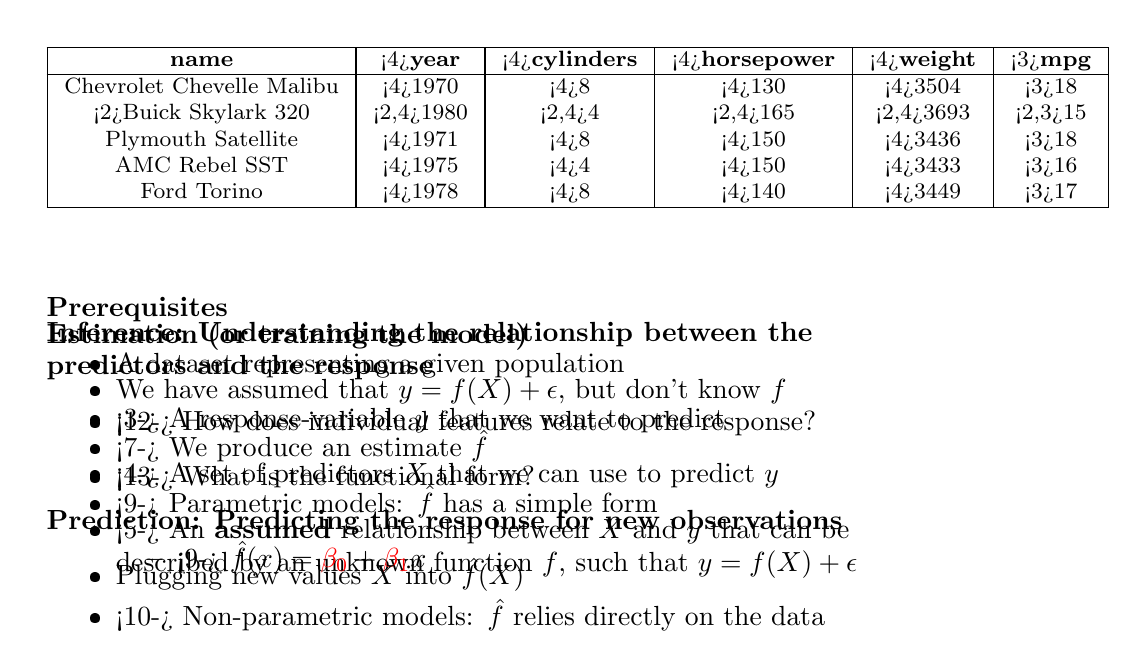
\begin{tikzpicture}
        \node[] at (-5.25, -3.5) {};
        \node[] at (5.25, 3.5) {};

        \visible<1-5>{
            \node[anchor=north west, ampersand replacement=\&, font=\footnotesize] at (-5.25, 3.5) {
                \begin{tabular}{|c|c|c|c|c|c|}
                    \hline
                    \textbf{name}&\alert<4>{\textbf{year}}&\alert<4>{\textbf{cylinders}}&\alert<4>{\textbf{horsepower}}&\alert<4>{\textbf{weight}}&\alert<3>{\textbf{mpg}}\\
                    \hline
                    Chevrolet Chevelle Malibu&\alert<4>{1970}&\alert<4>{8}&\alert<4>{130}&\alert<4>{3504}&\alert<3>{18}\\
                    \alert<2>{Buick Skylark 320}&\alert<2,4>{1980}&\alert<2,4>{4}&\alert<2,4>{165}&\alert<2,4>{3693}&\alert<2,3>{15}\\
                    Plymouth Satellite&\alert<4>{1971}&\alert<4>{8}&\alert<4>{150}&\alert<4>{3436}&\alert<3>{18}\\
                    AMC Rebel SST&\alert<4>{1975}&\alert<4>{4}&\alert<4>{150}&\alert<4>{3433}&\alert<3>{16}\\
                    Ford Torino&\alert<4>{1978}&\alert<4>{8}&\alert<4>{140}&\alert<4>{3449}&\alert<3>{17}\\
                    \hline
                \end{tabular}
            };
            \node[anchor=south west, text width=10.5cm] at (-5.25, -3.5) {
                \textbf{Prerequisites}
                \begin{itemize}
                    \item A dataset representing a given population
                    \item<3-> A response-variable $y$ that we want to predict
                    \item<4-> A set of predictors $X$ that we can use to predict $y$
                    \item<5-> An \textbf{assumed} relationship between $X$ and $y$ that can be described by an unknown function $f$, such that $y=f(X) + \epsilon$
                \end{itemize}
            };
        }
        \visible<6>{
            \node[] at (0, 1.75) {
                \usebox{\mpgpoints}
            };
        }
        \visible<7,9,11,13,15>{
            \node[] at (0, 1.75) {
                \usebox{\mpglinear}
            };
        }
        \visible<8,14>{
            \node[] at (0, 1.75) {
                \usebox{\mpgsquared}
            };
        }
        \visible<10>{
            \node[] at (0, 1.75) {
                \usebox{\mpgnonparametric}
            };
        }
        \visible<6-10>{
            \node[anchor=north west, text width=10.5cm] at (-5.25, 0) {
                \textbf{Estimation (or training the model)}
                \begin{itemize}
                    \item We have assumed that $y=f(X) + \epsilon$, but don't know $f$
                    \item<7-> We produce an estimate $\hat{f}$
                    \item<9-> Parametric models: $\hat{f}$ has a simple form
                    \begin{itemize}
                        \item<9-> $\hat{f}(x) = {\color{red}\beta_0} + {\color{red}\beta_1} x$
                    \end{itemize}
                    \item<10-> Non-parametric models: $\hat{f}$ relies directly on the data
                \end{itemize}
            };
        }
        \visible<12>{
           \node[] at (0, 1.75) {
               \usebox{\mpglinearhighlight}
           };
        }
        \visible<11-17>{
            \node[anchor=north west, text width=10.5cm, align=flush left] (inference) at (-5.25, 0) {
                \textbf{Inference: Understanding the relationship between the predictors and the response}
                \begin{itemize}
                    \item<12-> How does individual features relate to the response?
                    \item<13-> What is the functional form?
                \end{itemize}
            };
        }
        \visible<14-17>{
            \node[anchor=north west, text width=10.5cm, align=flush left] at (inference.south west) {
                \textbf{Prediction: Predicting the response for new observations}
                \begin{itemize}
                    \item Plugging new values $X$ into $\hat{f}(X)$
                \end{itemize}
            };
        }
        \visible<16>{
            \node[] at (0, 1.75) {
                \usebox{\mpgcalculation}
            };
        }
        \visible<17>{
            \node[] at (0, 1.75) {
                \usebox{\mpgyhat}
            };
        }
        % \visible<7>{
        %     \node[] at (0, 0) {
        %         Prediction and inference
        %     };
        % }
        % \visible<8>{
        %     \node[] at (0, 0) {
        %         Example
        %     };
        % }
        % \visible<9>{
        %     \node[] at (0, 0) {
        %         Metrics
        %     };
        % }
    \end{tikzpicture}
\end{frame}

